\documentclass[10pt,a4paper]{article}
\usepackage[utf8]{inputenc}
\usepackage[english]{babel}
\usepackage[T1]{fontenc}
\usepackage{amsmath}
\usepackage{amsfonts}
\usepackage{amssymb}
\usepackage{subcaption}
\usepackage{makeidx}
\usepackage{graphicx}
\usepackage{fourier}
\usepackage{listings}
\usepackage{color}
\usepackage{hyperref}
\usepackage[left=2cm,right=2cm,top=2cm,bottom=2cm]{geometry}
\author{Tommy Müller, Marcus Dittrich, Vincent Noculak}
\title{Quadrupol-Massenfilter}


\begin{document}


\section{Auswertung}

Zur Auswertung der Daten wurde Peak-o-Mat verwendet. Im Programm haben wir den Nullpunkt angepasst und den Sattel entfernt(< 3 u/e). Da der Massenfilter eine endliche Länge besitzt, werden kleine m/q in diesem Rauschen dargestellt. Bei kleinen Massen ist die Schwingung innerhalb des Quadrupolmassenfilters klein und damit die Spannungen klein. Der Massenfilter schafft es nicht für endlich viele Schwingungen unerwünschte Massen heraus zu filtern. Peak-o-Mat lieferte dann die Maxima und führte zu den Tabellen \ref{argtab},\ref{acetab} und \ref{ethatab}. Die Partialdrücke würde aus dem Verhältnis der Peaks zueinander errechnet, dabei auftretende Prozente wurden gerundet. Der Ausgangsdruck war immer 1.0 *$10^{-5}$. Dies änderte sich nur bei Argon auf 9,6*$10^{-6}$. Daher ist der Fehler maximal 4 \% der Partialdrücke. Bei Ethanol und Acethon hat der Druck sich nicht verändert.
Wir untersuchten zuerst Argon, dann Acethon und zum Schluss Ethanol. Diese Reihenfolge könnte bei der nachfolgenden Messung, durch nicht 100 \% entlüften, einfluss haben.


\begin{figure}[h]
	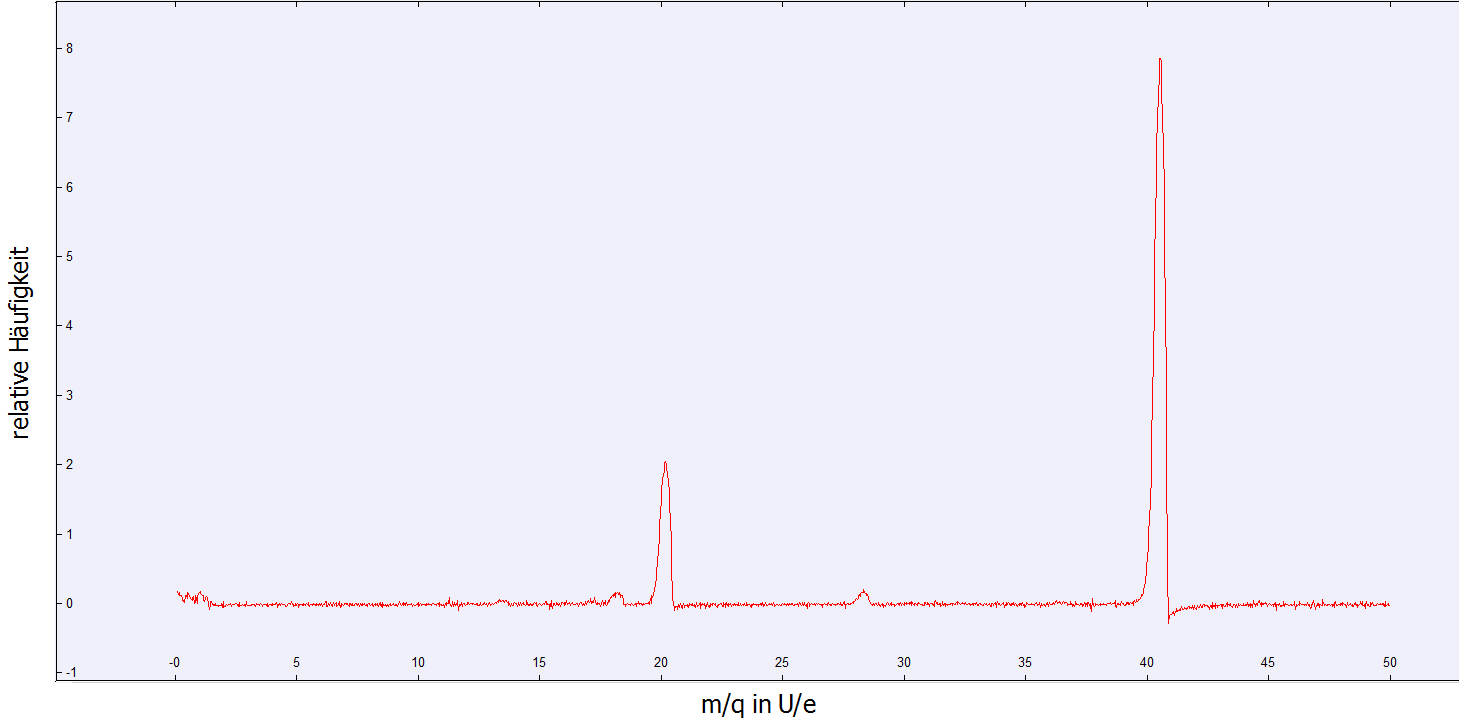
\includegraphics[scale = 0.2]{argon1.png}
	\centering
	\caption{Quadrupolmessung von Argon}
	\label{arg}
\end{figure}

\begin{figure}[h]
	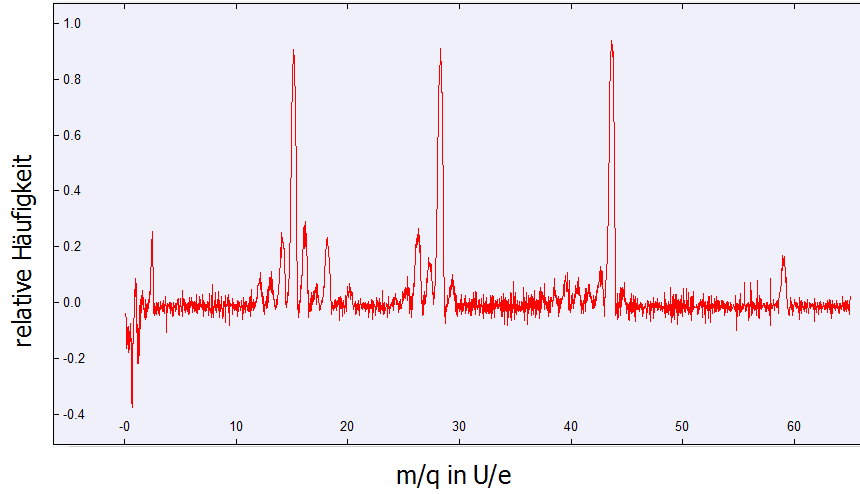
\includegraphics[scale = 0.3]{acethon1.png}
	\centering
	\caption{Quadrupolmessung von Acethon}
	\label{arg}
\end{figure}

\begin{figure}[h]
	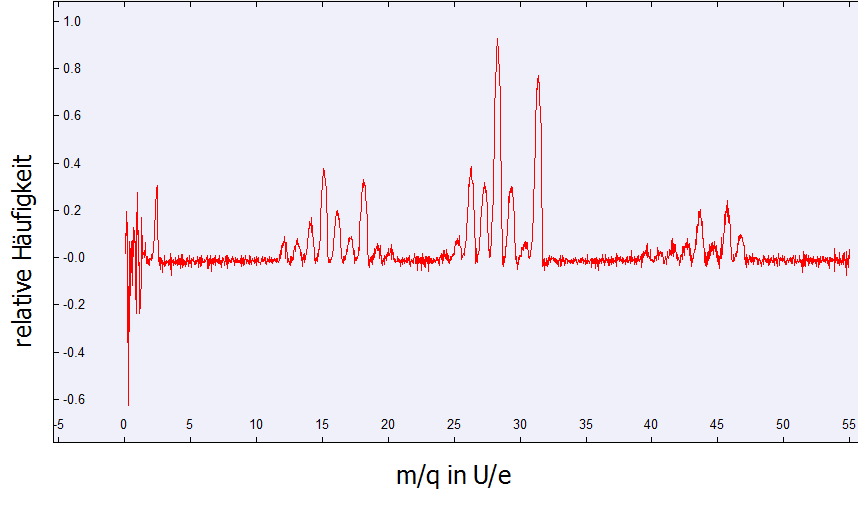
\includegraphics[scale = 0.3]{ethanol1.png}
	\centering
	\caption{Quadrupolmessung von Ethanol}
	\label{arg}
\end{figure}

\begin{figure}[h]
	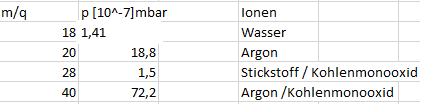
\includegraphics[scale = 0.5]{argontab.png}
	\centering
	\caption{Quadrupolmessung von Argon, mögliche Ionen}
	\label{argtab}
\end{figure}

\begin{figure}[h]
	\includegraphics[scale = 0.5]{acethontab.png}
	\centering
	\caption{Quadrupolmessung von Acethon, mögliche Ionen}
	\label{acetab}
\end{figure}

\begin{figure}[h]
	\includegraphics[scale = 0.5]{ethanoltab.png}
	\centering
	\caption{Quadrupolmessung von Ethanol, mögliche Ionen}
	\label{ethatab}
\end{figure}

\section{Diskussion}

Argon kann nicht innerhalb des Versuchsaufbau "zerfallen", wobei hingegen Acethon und Ethanol in Untergruppen zerfallen kann z.B. in Methan Acethylen Athylen, Ammoniak, Methanol, Prophan, Prophen... dazu kommt noch Luftbestandteile wie Kohlenmonooxid, Stickstoff, Sauerstoff und Neon. Diese doch lange Liste führ zu einer Auswahl an Ionen die wir detektiert haben. Der Fehler der Partialdrücke ist auf 4\% geschätzt da nur bei einer Messung der Druck abgefallen ist.


\end{document}